\documentclass[tikz,border=10pt]{standalone}
\usepackage{tikz}
\usetikzlibrary{angles,quotes,calc}

\begin{document}
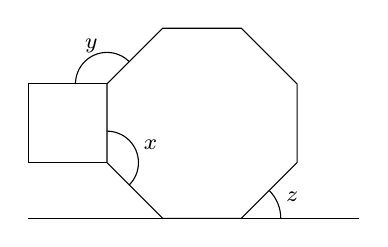
\begin{tikzpicture}[scale = 1]
    % Initial point
    \coordinate (A) at (0,0);
    % Draw octagon
    \draw (A) -- ++(0:1cm) coordinate(K) -- ++(45:1cm) coordinate (L) -- ++(90:1cm)  -- ++(135:1cm) -- ++(180:1cm) coordinate (D) -- ++(225:1cm) coordinate (B) -- ++(270:1cm) coordinate (E) -- cycle;
    % Draw square to the left of the octagon
    \draw (B) -- ++(180:1cm) coordinate (C) -- ++ (270:1cm) -- ++(0:1cm);

    % Draw base line
    \draw (C |- 52,0) -- (2.5,0);
    \coordinate (M) at (2.5,0);
    
    % Draw the angle between lines
    \pic [draw, "\footnotesize $z$ ", angle eccentricity=1.4, angle radius=0.5cm] {angle = M--K--L};
    \pic [draw, "\footnotesize $y$", angle eccentricity=1.3, angle radius=0.4cm] {angle = D--B--C};
    \pic [draw, "\footnotesize $x$", angle eccentricity=1.5, angle radius=0.4cm] {angle = A--E--B};
    
\end{tikzpicture}
\end{document}

